%\documentclass[a4paper,oneside,12pt]{report} % n.pag scritto in basso
\documentclass[a4paper,oneside,11pt]{book}   
% Size and sheet settings
\usepackage[a4paper, top=3.5cm, bottom=3.5cm, left=2.5cm, right=3cm, heightrounded, bindingoffset=5mm]{geometry}

% Input encoding
\usepackage[utf8]{inputenc} 
\usepackage[T1]{fontenc}
% Per gestire le immagini
\usepackage{graphicx}  
% Per inserire margini laterali
\usepackage{scrextend} 
% Per fare la title page con immagine
\usepackage{titling}  
% For special styles (code)
\usepackage[dvipsnames]{xcolor}
\colorlet{punct}{red!60!black}
\definecolor{background}{HTML}{EEEEEE}
\definecolor{delim}{RGB}{20,105,176}
\colorlet{numb}{magenta!60!black}
\usepackage{listings}

% To set depth table of contents
\setcounter{tocdepth}{4}

%% TABLES
% Utile per usare H per svuotare la cache dei floating objects come le table
\usepackage{float}     
% Necessario per rappresentare tabelle su più pagine
\usepackage{longtable} 
% Necessario per creare un nuovi tipi di colonna per le tabelle
\usepackage{array}     
\usepackage{tabu}

% Special table columns to center between cells
\newcolumntype{X}[1]{>{\centering\arraybackslash}p{#1}}
\newcolumntype{C}[1]{>{\centering\arraybackslash}m{#1}}
\newcolumntype{P}[1]{>{\arraybackslash}p{#1}}
\newcolumntype{H}[1]{>{\arraybackslash}m{#1}}

% Aggiunge funzionalità alle captions
\usepackage{caption}   
% Distacca le caption dalle table (verticalmente)
\captionsetup[table]{skip = 8pt} 
% Default: 6pt - Margine laterale  tra le celle delle tabelle
\setlength{\tabcolsep}{10pt}      
% Default: 1 - Margine verticale tra le celle delle tabelle
\renewcommand{\arraystretch}{1.7} 

% Multicolumn sections
\usepackage{multicol}

% Clickable references
\usepackage{hyperref} 
\hypersetup{
    colorlinks=true,
    linkcolor=blue,
    filecolor=black,      
    urlcolor=cyan,
    pdftitle={CLup - Acceptance Testing Document}, % Title of output file
    pdfpagemode=FullScreen,            % To open in fullscreen
}
% Command for two-part captions for tables/pictures
\newcommand{\captionatd}[2]{\caption{#1}\par\begin{center}\vspace{-.01\textheight}\small#2.\end{center}}
% Command for correctly spaced coloured text
\newcommand{\red}[1]{\begingroup\color{punct}#1\endgroup}

\title{\LARGE{CLup -- Acceptance Testing Document}}
\author{Vincenzo Riccio, Giancarlo Sorrentino, Emanuele Triuzzi}
\date{14th February, 2021}
\begin{document}

\begin{titlingpage} 
    \begin{center}
        
\includegraphics[height=0.52\linewidth]{pictures/polimi}\\ % Logo
        \begin{large}
            Software Engineering 2 \\
            A.Y. 2020-2021\\
        \end{large}
        \vspace{4cm} % Spaziatura verticale
        \begin{large} 
            \textbf{\thetitle} \\
        \end{large}
        \vspace{0.7cm}
        \theauthor
        \par\small{\url{https://github.com/SirGian99/RiccioSorrentinoTriuzzi}} \begin{center}
            \par\par \begin{center}\large{\textit{Project Tested}}\end{center} \url{https://github.com/AlessioBatta/BattagliaBelliniPasini}\par\par
        \end{center}
        
        \vspace{6.2cm} % Spaziatura verticale
        \thedate
    \end{center}
\end{titlingpage}

\newpage
\begin{table}[H]
    \begin{tabu} to \textwidth { X[0.3,r,p] X[0.7,l,p] }
        \hline
        \textbf{Deliverable:}   & ATD\\
        \textbf{Title:}         & Acceptance Testing Document \\
        \textbf{Authors:}       & Vincenzo Riccio, Giancarlo Sorrentino, \newline Emanuele Triuzzi \\
        \textbf{Version:}       & 1.0 \\ 
        \textbf{Date:}          & 14th February, 2021 \\
        \textbf{Download page:} & https://github.com/SirGian99/RiccioSorrentinoTriuzzi \\
        \textbf{Copyright:}     & Copyright © 2021, Vincenzo Riccio, Giancarlo Sorrentino, Emanuele Triuzzi -- All rights reserved \\
        \hline
    \end{tabu}
\end{table}

%\href{run:../DeliveryFolder/RASD2.pdf}{Requirement Document}
%\ref{section:design_decisions}

\pagenumbering{roman}
\tableofcontents
\newpage
\pagenumbering{arabic}

\chapter{Introduction}
    \section{Purpose}
    The document purpose is to validate and test a project implemented by another group of the Software Engineering 2 course. \par
    In particular, the authors of the analysed project are:
    \begin{itemize}
        \item Alessio Battaglia;
        \item Simone Bellini;
        \item Samuele Pasini.
    \end{itemize}
    Their repository is reachable through this URL: \par
    \url{https://github.com/AlessioBatta/BattagliaBelliniPasini}.
    
    \section{Overview}
    The analysis of the project has been performed by accurately reading the documents produced by the team while paying attention to the consistency between them. \par
    Then, we prepared a working configuration of our machines following the installation instructions included in the Implementation and Testing Document. \par
    While doing so, it has been tracked any difficulty found. \par
    Once the software was correctly configured, it has been properly examined by identifying which requirements it does satisfy and which does not. Moreover, the provided test cases have been run in order to evaluate the correctness of the implementation. \par
    At the end, a full end to end test has been performed in order to test the general behaviour of the software, while looking at the use cases defined in the RASD and at the decisions taken in the DD.
    
    \section{Revision history}
    \begin{itemize}
        \item[\textbf{1.0}] First version of the document. (14th February, 2021)
    \end{itemize}
    
    \section{Reference documents}
    \begin{itemize}
        \item Implementation and Testing assignment A.Y. 2020-2021;
        \item Teaching material provided by professors Matteo Rossi and Elisabetta Di Nitto;
        \item Requirement Analysis Specification Document, Design Document, Implementation and Testing Document of the team.
    \end{itemize}
    
    \section{Document structure}
    The reference structure used for the document is an adapted version of the one suggested by professor Matteo Rossi of Politecnico of Milan.
    
    \subsubsection{Chapter 1}
    The first chapter provides an introduction to the document and introduces what has been done and evaluated in the project being tested.
    
    \subsubsection{Chapter 2}
    The second chapter describes how the installation setup has been made following the installation instructions included in the ITD. 

    \subsubsection{Chapter 3}
    Chapter 3, which is the core of this document, focusses on acceptance tests: the software is tested with tests proposed by the group, by following test cases presented in the RASD, and by specific cases that are considered interesting. While doing so, also the performance of the tests are taken into account.
    
    \subsubsection{Chapter 4}
    The fourth chapter concludes the document summarizing and adding further comments about the work done by the group in question.
    
    \subsubsection{Chapter 5}
    Last chapter contains references to the tools and resources used to implement the system and to write the document.
    
\chapter{Installation setup}
    The installation guide provided in the ITD is quite detailed. We really appreciated the presence of figures describing the installation steps. However, it is very platform dependent and the part about Docker is incomplete. \par For this reason, we had some troubles while preparing a Mac environment for running the whole software, while with Windows the guide is nearly perfect, with the already mentioned exception of the Docker part. \par
    Thus, the following setup refers to the software installation on macOS.

    \section{Server installation}
    We started installing all the needed software to run the project. The first installed software was JDK 13. We downloaded the OpenJDK version from the Java JDK Archive website (included in the references), since the URL they provided redirects to JDK 15. We properly installed and configured it, making it available to the entire OS. \par
    Since MySQL Server and Workbench were already installed on our machines, we only imported the CLup database dump. A little remark on that part of the guide: they do not specify a version to install, and we found some collation problems with MySQL 5.x. \par
    Then we downloaded and installed Eclipse and all the plugins and dependencies mentioned in the ITD. The Enterprise version of Eclipse already includes Maven, so there was no need to configure it. \par
    After opening the project, we edited the configuration file as stated in the guide in order to set the correct parameters allowing the connection to the MySQL DB instance. \par
    However, in order to use the provided \texttt{.jar} artifact, the steps described in the ITD are not totally right. In fact, they suggest editing the \texttt{application.properties} file located in the jar’s same folder as done in Eclipse, but it is not possible to directly execute the jar artifact without adding their same user to MySQL. \par
    We ended the installation of the backend software by installing Docker. Here is where we found some difficulties: the installation guide is not so detailed about it and we initially found some troubles while running some containers-dependent tests.

\newpage
    \section{Client installation}
    The mobile application required only Flutter and Android Studio in order to run it. We downloaded and installed them according to the official guides for macOS, and no problems were encountered. We configured them according to the guide they provided in the ITD, needing to adapt only the environment variables section for macOS (we followed the official Flutter installation guide for macOS, see references). \par
    However, since Android Studio is quite demanding in terms of hardware specifications,we found some difficulties running the device simulator. \par
    For this reason, an APK would have been really appreciated in order to test the app on a proper device instead of a slow simulator (they state that the server must run on the same machine, but with a proper configuration no problems would arise).

\chapter{Acceptance test}
    We started the acceptance test looking at the tests included in the implementation. We ran them many times to check they never fail. However, even if they suggest to never execute them near midnight, one test (\texttt{createTicketTest}) fails even at 19:00. Of course, it is just a little remark, since they offer a huge variety of tests.
    \section{Goals}
    \begin{longtable}[c] { |>{\centering\arraybackslash}C{0.08\textwidth}|>{\arraybackslash}H{0.47\textwidth}|>{\centering\arraybackslash}H{0.23\textwidth}| }
        \hline
        \textbf{G1} & Limit the total number of customers in a shop to a certain amount & \textit{Achieved} \\ \hline
        \textbf{G2} & Prevent the formation of physical queues and gatherings outside & \textit{"To prevent" is not possible, but beside that, achieved} \\ \hline
        \textbf{G3} & Allow customers to enter when the number of people inside a shop is fewer than a certain amount & \textit{Achieved} \\ \hline
        \textbf{G4} & Allow the customers to enter when it is their turn & \textit{Achieved} \\ \hline
        \textbf{G5} & Block the customers’ entrance when it is not their turn & \textit{Achieved} \\ \hline
        \textbf{G6} & Allow the customers to know when it is their turn & \textit{Achieved} \\ \hline
        \textbf{G7} & Allow customer to know the current situation of the queue before getting a ticket & \textit{Achieved} \\ \hline
        \textbf{G8} & Allow the user to manage booking visits to a supermarket at a certain time/day & \textit{Achieved, but with the choice made, each customer can have at most one booking} \\ \hline
        \textbf{G9} & Reduce the number of bookings without entrance & \textit{Achieved} \\ \hline
        \textbf{G10} & Let customers who do not have the application to still have an access & \textit{Proxy not implemented} \\ \hline
        \textbf{G11} & Allow the user to see if there are advantageous alternatives to their current choice & \textit{Alternatives not implemented} \\ \hline
        \caption{Goals achieved}
        \label{table:goals}
    \end{longtable} 
    
    \section{Requirements}
    \begin{longtable}[c] { |>{\centering\arraybackslash}C{0.08\textwidth}|>{\arraybackslash}H{0.47\textwidth}|>{\centering\arraybackslash}H{0.23\textwidth}| }
        \hline
        \textbf{R1} & A customer should be allowed to sign up to use the CLup application & \textit{Satisfied} \\ \hline
        \textbf{R2} & A user should be allowed to sign in by inserting his access data (username and password) & \textit{Satisfied} \\ \hline
        \textbf{R3} & Users should be allowed to make an online booking & \textit{Satisfied} \\ \hline
        \textbf{R4} & CLup system should check if users already have a booking before giving them one & \textit{Satisfied, but as a consequence it’s not possible to let customers book more than one visit to a store at the time} \\ \hline
        \textbf{R5} & CLup system should check if there are free slots before let the user makes a booking & \textit{Satisfied} \\ \hline
        \textbf{R6} & A user should be allowed to delete a previous booking & \textit{Satisfied} \\ \hline
        \textbf{R7} & If a user makes multiple bookings without going at the supermarket, the service should be temporarily deactivated & \textit{Not implemented} \\ \hline
        \textbf{R8} & Users should be allowed to take a virtual ticket & \textit{Proxy not implemented} \\ \hline
        \textbf{R9} & Customers should be allowed to take a physical ticket from the ticket generator outside the store & \textit{Satisfied (only for app-customers)} \\ \hline
        \textbf{R10} & CLup system should check if users already have a ticket before giving them one & \textit{Satisfied} \\ \hline
        \textbf{R11} & There should be a virtual lining up system for those who take a ticket & \textit{Satisfied} \\ \hline
        \textbf{R12} & A customer should be allowed to see the last called number & \textit{Satisfied} \\ \hline
        \textbf{R13} & A user should be allowed to see the approximate waiting time before getting a ticket & \textit{Satisfied} \\ \hline
        \textbf{R14} & Every shop should show the approximate waiting time at the entrance to all customers who wants to get a ticket & \textit{Satisfied (only for app-customers)} \\ \hline
        \textbf{R15} & CLup system should allow store manager to insert the parameters of his store when he adheres to the service & \textit{Manager not implemented} \\ \hline
        \textbf{R16} & The FMS should check if an entry code is associated to a booking or a ticket & \textit{Satisfied} \\ \hline
        \textbf{R17} & If the FMS status is CLOSED, the gates should be blocked for everyone & \textit{Satisfied} \\ \hline
        \textbf{R18} & If the FMS status is OPEN\textunderscore FOR\textunderscore BOOKINGS, the gates should be blocked for the customer with a ticket and unlocked for the one with a booking & \textit{Satisfied} \\ \hline
        \textbf{R19} & If the FMS status is OPEN, the gates should be unlocked for everyone with a valid ticket/booking & \textit{Satisfied} \\ \hline
        \textbf{R20} & For every entrance or exits, the status of the FMS should be recalculated & \textit{Satisfied} \\ \hline
        \textbf{R21} & CLup system should detect supermarkets near the chosen one with their relative queue status & \textit{Alternatives not implemented} \\ \hline
        \textbf{R22} & Store managers should be allowed to see the situation in their store, with trends, booking and queue status & \textit{Manager not implemented} \\ \hline
        \textbf{R23} & Store managers should be allowed to update their store parameters & \textit{Manager not implemented} \\ \hline
        \caption{Requirements}
        \label{table:requirements}
    \end{longtable} 
    
    The requirements which in the ITD they state to satisfy are really satisfied by the prototype. However, they do not provide any detail on the non-functional requirements satisfied (if there are).

    
    \section{Use case tests}
    In order to evaluate how to prototype satisfies the goals described in the Requirement Analysis Specification Document, we performed a deep end-to-end test to check whether any functions could exhibit any problem in its correct functioning. \par
    The following table shows which of the use cases described in the RASD are foreseen by the prototype. \par
    All the implemented use cases are fully working and coherent with the RASD.

    \begin{longtable}[c] { |H{0.40\textwidth}|>{\em}C{0.30\textwidth}| }
        \hline
        Sign up & Implemented \\ \hline
        Sign in & Implemented \\ \hline
        Logout & Implemented\\ \hline
        Take a ticket & Implemented\\ \hline
        Select a supermarket to line-up & Implemented\\ \hline
        Ask a suggestion for a line-up & Not implemented\\ \hline
        Book a visit & Implemented \\ \hline
        Select slots for booking & Implemented \\ \hline
        Ask suggestion for a booking & Not implemented\\ \hline
        Delete a booking & Implemented \\ \hline
    \caption{Use cases implementation}
    \label{table:use_cases}
    \end{longtable}
        
    
    Regarding the product functions listed in the RASD, the first three (\textit{Virtual ticket handling, Book a visit to a supermarket and Manage the flow of customers}) are planned in the ITD and correctly implemented in the prototype. Moreover, the \textit{State diagram for app users} (\textit{RASD, Figure 2}) is respected too.


    \newpage
    \section{Unit and Integration testing}
    To check the correctness of the implemented code, we also run all the tests included in the project. The following table underlines the execution of the tests on our machines, and their relative time of execution.
    \begin{longtable}[c] { |H{0.55\textwidth}|>{\em}C{0.15\textwidth}| }
        \hline
        CLupApplicationTests & 0,322 s \\ \hline
        BookingRequestTest & 0,207 s\\ \hline
        SignupRequestTest & 0,230 s\\ \hline
        OpeningDayServiceTest & 0,362 s\\ \hline
        StoreServiceTest & 0,184 s\\ \hline
        SlotServiceTest & 0,053 s\\ \hline
        TicketServiceTest & 0,184 s\\ \hline
        BookingServiceTest & 0,145 s\\ \hline
        AuthServiceTest & 0,108 s\\ \hline
        DayServiceTest & 3,182 s\\ \hline
        BookingMapperTest & 0,248 s\\ \hline
        TicketMapperTest & 0,257 s\\ \hline
        StoreMapperTest & 3,673 s\\ \hline
        CityRepositoryTest & 0,341 s\\ \hline
        StoreRepositoryTest & 0,257 s\\ \hline
        RegionRepositoryTest & 0,115 s\\ \hline
        DayRepositoryTest & 0,083 s\\ \hline
        SlotRepositoryTest & 0,220 s\\ \hline
        UserRepositoryTest & 0,159 s\\ \hline
        ProvinceRepositoryTest & 0,106 s\\ \hline
        TicketRepositoryTest & 0,250 s\\ \hline
        OpeningDayRepositoryTest & 0,064 s\\ \hline
        BookingRepositoryTest & 0,139 s\\ \hline
    \caption{Results of the tests performed using JUnit 5}
    \label{table:tests}
    \end{longtable}
    
\chapter{Conclusions and further comments}
    The group did a very good job, since as said before the prototype satisfies the main requirements and it is very complete. Furthermore, the mobile application prototype follows quite perfectly the mock-ups provided through the RASD and DD and it even includes remote notifications through Firebase. \par
    The code quality is also very good, following nice design patterns, and coherent with the architecture presented in the Design Document. Furthermore, it is also sufficiently documented. \par
    It is glaring that the group worked with a lot of commitment and competence.
    Also, the group showed great disposability whenever needed in order to solve the encountered problems, in particular during the installation phase. \par
    However, these are some last remarks regarding the implemented functionalities:
    \begin{itemize}
        \item The first remark, that regards the entire project, is the absence of a feature specified in the assignment, which is the one that allows users to specify which kind of products they intend to buy when placing a booking, in order to better handle the influx of people in the store.
        \item The second remark regards the “easy to use” feature of the application. The application appears to be very intuitive. In fact, as shown in the picture below, its main functionalities are handly shown just after the sign in process.
        \begin{figure}[H]
            \centering
            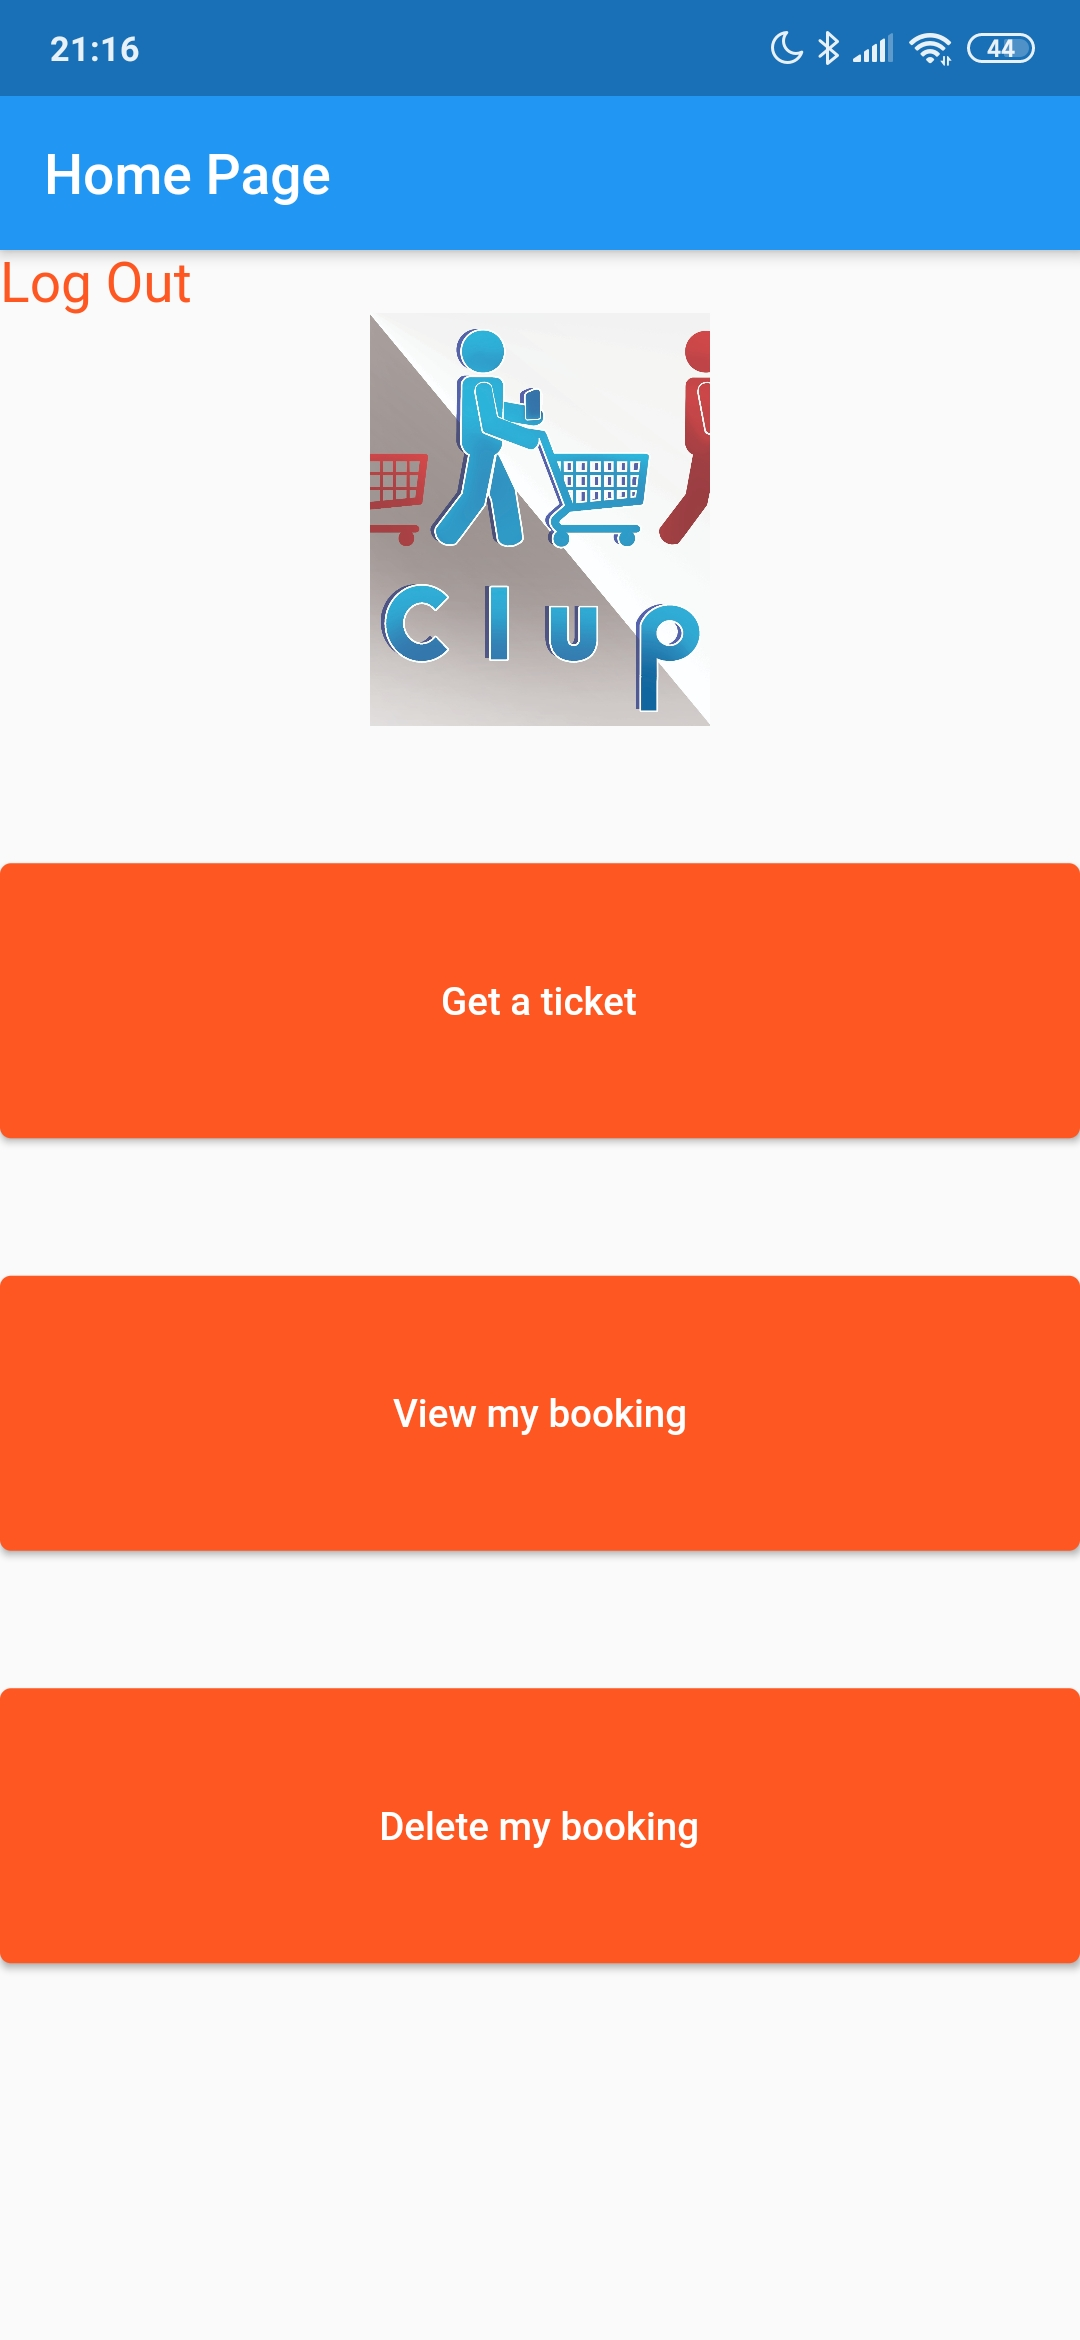
\includegraphics[width=.4\textwidth, height=\textheight, keepaspectratio]{pictures/screenshots/home_view.jpg}
            \caption{Home view}
            \label{figure:home_view}
        \end{figure}
        \item However, one remark on the application is the poor, in our opinion, handling of regions, provinces and cities. In fact, as shown in the picture below, it is quite unintuitive the selection of the previous specified fields when selecting a store. \par
        \begin{figure}[H]
            \centering
            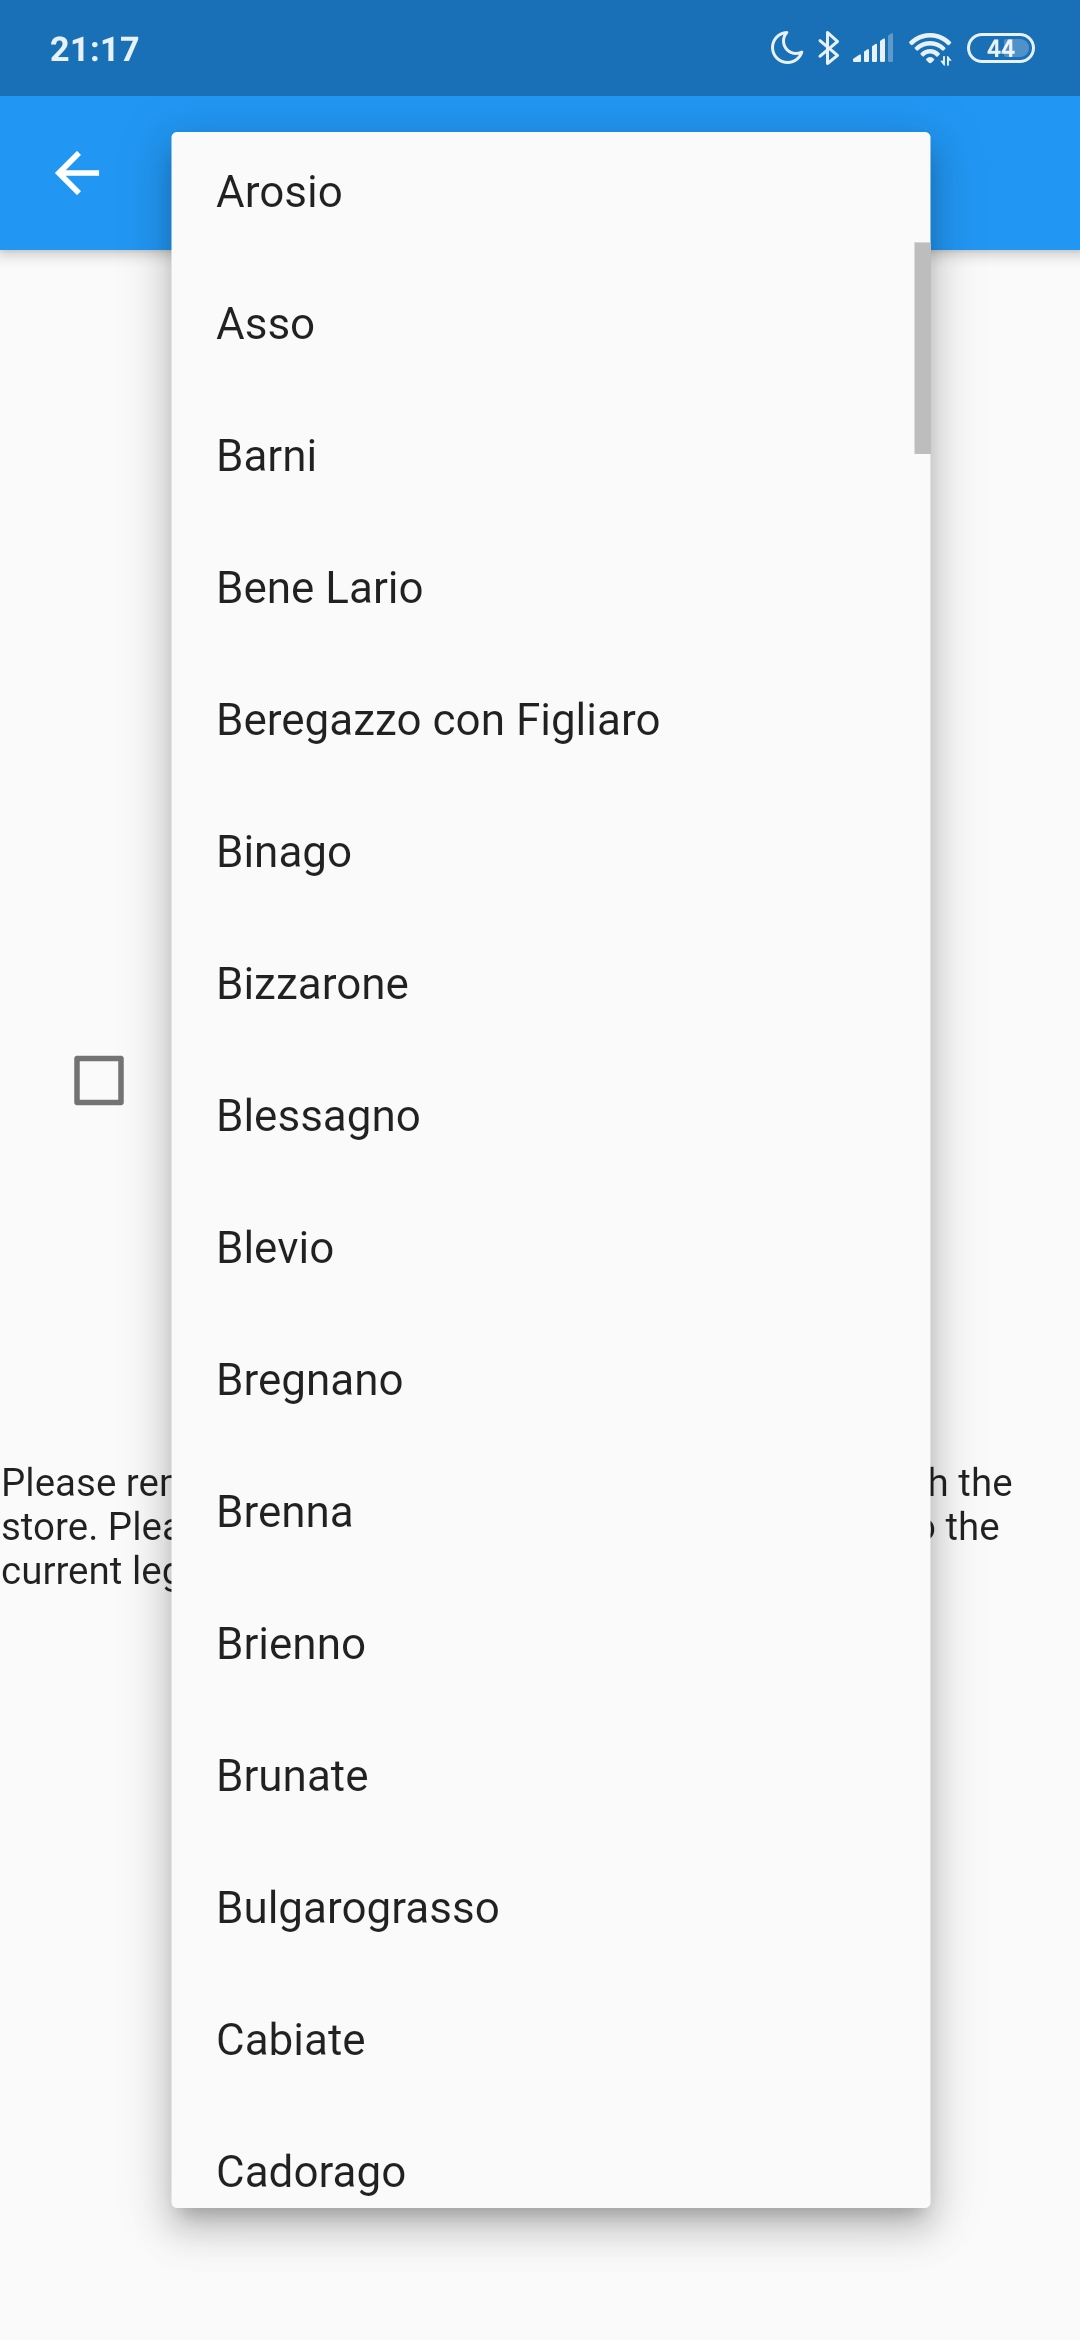
\includegraphics[width=.4\textwidth, height=\textheight, keepaspectratio]{pictures/screenshots/city_selector.jpg}
            \caption{City selector}
            \label{figure:city_selector}
        \end{figure}
        The application shows, without any logic, all the different possible values for the three fields, even if no store is available in the selected location: trying to find the available stores is indeed quite difficult among all the “useless” possibilities. \par
        Furthermore, from a customer’s point of view, it would have been great to know the working hours of a store before trying to place a booking or to get a ticket. It can be stressful finding a store among all the possible cities only to discover that it is currently closed.
        \item A last negative remark concerns the entity-relationship and logic shema. The proposed and implemented one is not so much scalable, since, for example, the table “day” should contain all the possible days in which a user can book a visit to a store. Taking into consideration the “test” database, it is impossible to book a visit to any store for a day after the 26/02/2021. \par To allow users to make a reservation to any store for any other day after the 26/02, those days should be manually inserted in the “day” table. This solution is quite “raw”, and could have been better implemented without the need to create a “day” table.
    \end{itemize}

    
\chapter{References}
    This chapter contains references to the tools and resources used during the writing of the document. \par
    \begin{itemize}
        \item \textit{Java Development Kit} 
        
        \url{https://jdk.java.net/archive/}
        \item \textit{Eclipse} 
        
        \url{https://www.eclipse.org/downloads/packages/}
        \item \textit{Flutter installation on MacOS} 
        
        \url{https://flutter.dev/docs/get-started/install/macos}
        \item \textit{Apache Maven} 
        
        \url{https://maven.apache.org/guides/}
        \item \textit{Android Studio}
        
        \url{https://developer.android.com/studio}
        \item \textit{Docker}
        
        \url{https://www.docker.com/get-started}
        
        \item \textit{JUnit 5} 
        
        \url{https://junit.org/junit5/}
    \end{itemize}

\listoftables
\listoffigures

\end{document}






































